\chapter{Learning Prob. Submodular Models} \label{ch:genes}

\section{Introduction}
\todo{Learning: one of the main motivations of thesis}

\todo{Outline general approach and explain where sampling comes in}

\subsection{Modeling interaction of gene alterations in cancer patients}
\todo{Explain basic problem and why it is interesting for cancer research}

\todo{Previous approaches}

\todo{How we use PSMs for this}

\todo{Contributions and advantages over previous work}


\section{Sampling for Approximate Maximum Likelihood Learning}

\todo{derive ML equations}

Given a data set of $N$ sets, $\mathcal{D} \defeq (S_1,\ldots,S_N)$, $S_1,\ldots,S_N \subseteq V$, the log-likelihood of the model is
\begin{align*}
L(\btheta) &\defeq \sum_{i=1}^N \log p(S_i; \btheta)\\
           &= \sum_{i=1}^N \left( F(S_i; \btheta) - \log Z(\btheta) \right)\\
           &= \sum_{i=1}^N F(S_i; \btheta) - N \log Z(\btheta).
\end{align*}
The gradient of the log-likelihood with respect to the parameters $\btheta$ is
\begin{align*}
\nabla_{\btheta} L(\btheta) &= \sum_{i=1}^N \nabla_{\btheta} F(S_i; \btheta) - N \nabla_{\btheta} \log Z(\btheta)\\
                            &= \sum_{i=1}^N \nabla_{\btheta} F(S_i; \btheta) - N \frac{1}{Z(\btheta)} \nabla_{\btheta} Z(\btheta)\\
                            &= \sum_{i=1}^N \nabla_{\btheta} F(S_i; \btheta) - N \frac{1}{Z(\btheta)} \nabla_{\btheta} \sum_{S \subseteq V} \exp\left( F(S; \btheta) \right)\\
                            &= \sum_{i=1}^N \nabla_{\btheta} F(S_i; \btheta) - N \sum_{S \subseteq V} \frac{\exp\left( F(S; \btheta)\right)}{Z(\btheta)} \nabla_{\btheta} F(S; \btheta)\\
                            &= \sum_{i=1}^N \nabla_{\btheta} F(S_i; \btheta) - N \sum_{S \subseteq V} p(S; \btheta) \nabla_{\btheta} F(S; \btheta)\\
                            &= \sum_{i=1}^N \nabla_{\btheta} F(S_i; \btheta) - N\,\E_{p}\left[ \nabla_{\btheta} F(S; \btheta) \right]
\end{align*}

\todo{Explain the role of sampling.}

\paragraph{Gradients of the \fldc{} model.}
Since we will be focusing on the \fldc{} model for the remainder of this chapter, we derive here the gradients with respect to its parameters.
As a reminder, the \fldc{} model is defined via the following function \cite{djolonga16mixed},
\begin{align*}
F(S; \bu, \bw, \bv) = \sum_{i \in S} u_i + \sum_{j=1}^{L} \left(\max_{i \in S} w_{ij} - \sum_{i \in S} w_{ij}\right) - \sum_{j=1}^{L} \left(\max_{i \in S} v_{ij} - \sum_{i \in S} v_{ij}\right).
\end{align*}
This function is differentiable everywhere except for a finite number of points, due to the presence of the two $\max$ operators.
For those points, we define subgradients that give equal contribution to all elements that belong to the corresponding $\argmax$.
In particular, for all $i \in V$, $j \in [L]$, we have
\begin{align*}
\nabla_{u_i} F(S; \bu, \bw, \bv) &= \ind[i \in S]\\
\nabla_{w_{ij}} F(S; \bu, \bw, \bv) &= \frac{\ind[i \in \argmax_{r \in S} w_{rj}]}{|\argmax_{r \in S} w_{rj}|} - \ind[i \in S]\\
\nabla_{v_{ij}} F(S; \bu, \bw, \bv) &= -\frac{\ind[i \in \argmax_{r \in S} v_{rj}]}{|\argmax_{r \in S} v_{rj}|} + \ind[i \in S].
\end{align*}
\citet{tschiatschek16} used an alternative set of subgradients, involving randomization over the choice of the $\argmax$ at each gradient step.
We have noticed that our choice often results in slightly improved learning performance in practice.


\subsection{Implementation details}
\todo{Projection to positive orthant; sparsity -- projection to L1-ball}

\section{Synthetic Data}
\todo{Show learning curve for small example}

\section{Real Cancer Data}

\subsection{Acute myeloid leukemia (AML)}

\begin{figure}[htb]
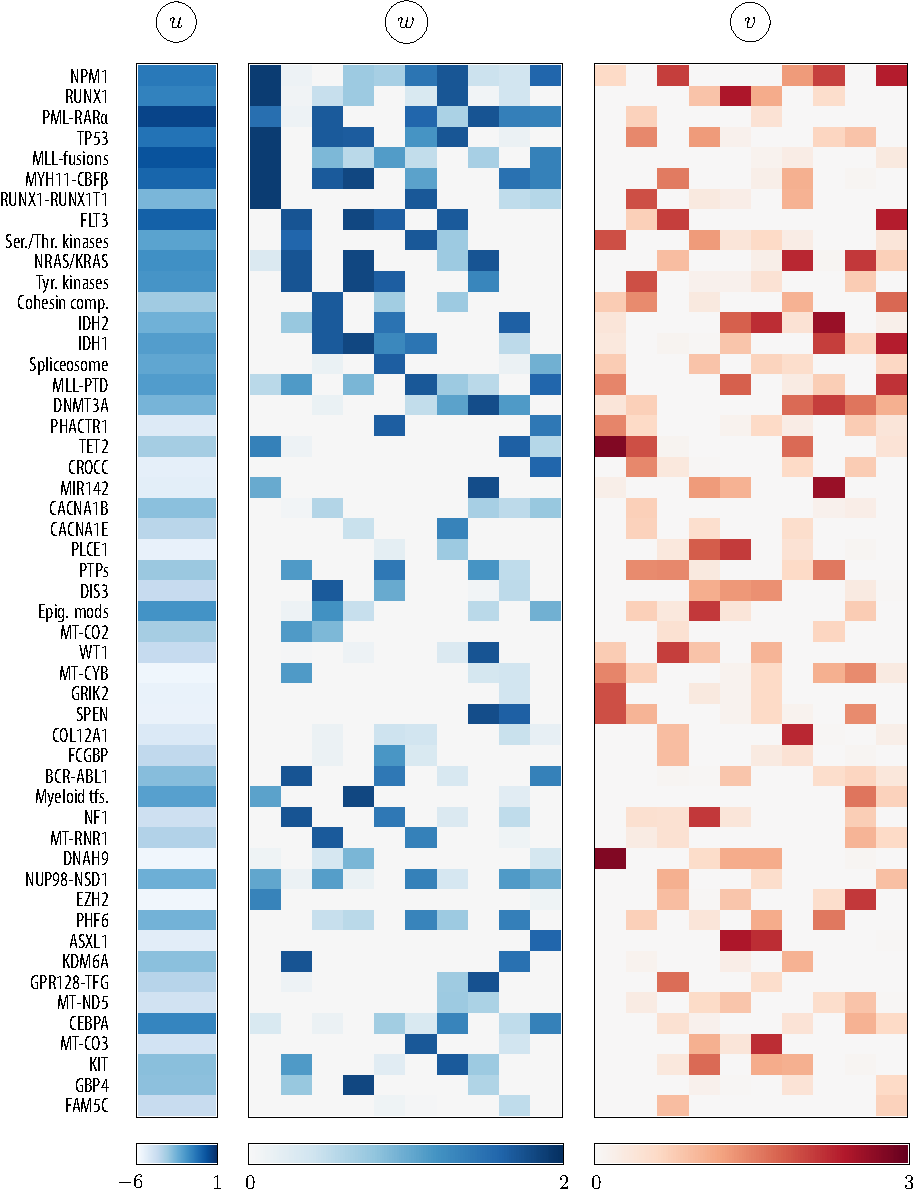
\includegraphics[width=\textwidth]{figures/genes/mat_aml.pdf}\\[2em]
\caption{Test}
\end{figure}

\begin{figure}[htb]
\centering
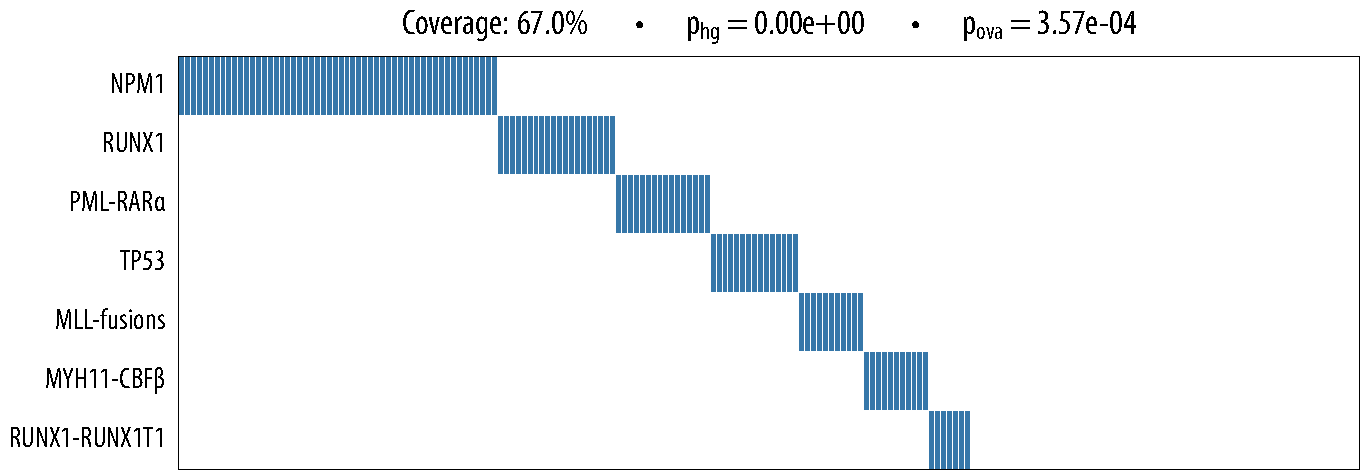
\includegraphics[width=\textwidth]{figures/genes/aml_1.pdf}\\[2em]
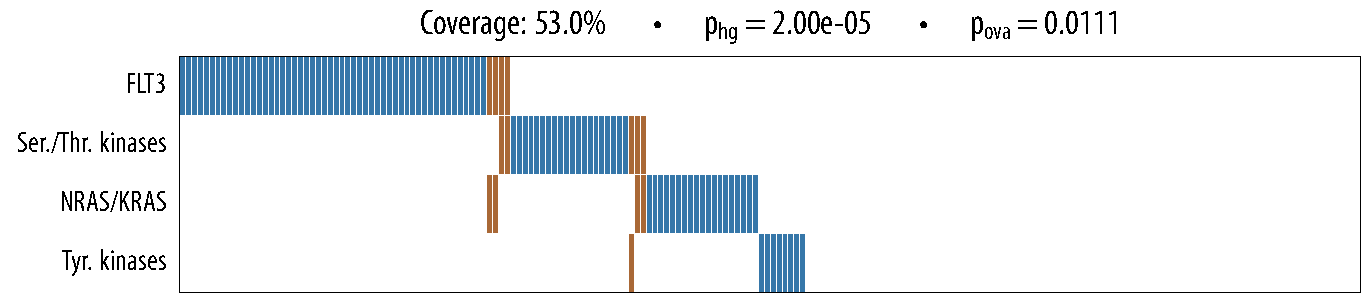
\includegraphics[width=\textwidth]{figures/genes/aml_2.pdf}\\[2em]
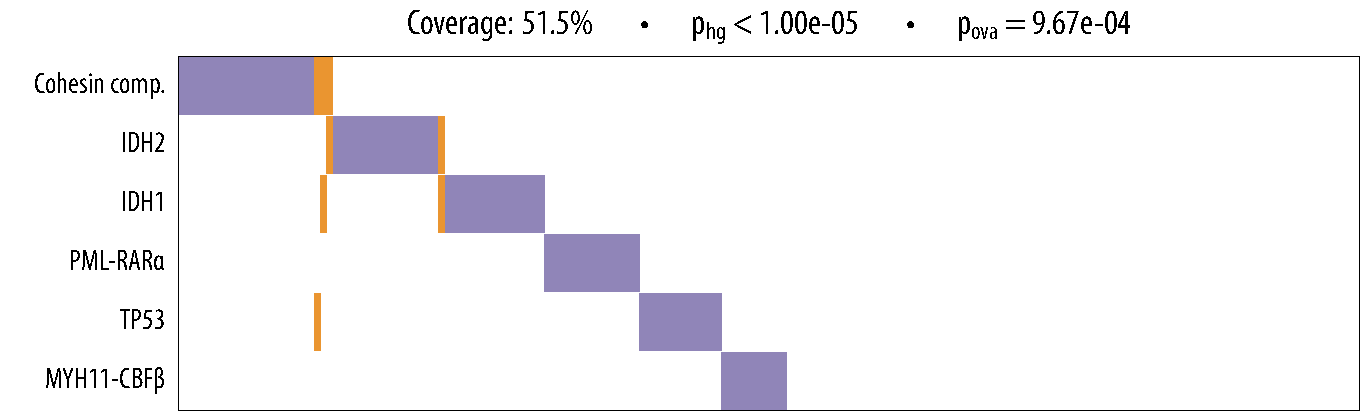
\includegraphics[width=\textwidth]{figures/genes/aml_3.pdf}\\[2em]
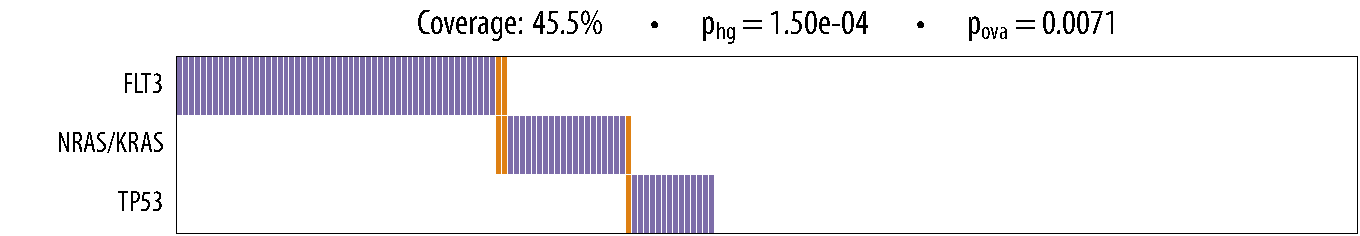
\includegraphics[width=\textwidth]{figures/genes/aml_4.pdf}\\[2em]
\caption{Test}
\end{figure}

\begin{figure}[htb]
\centering
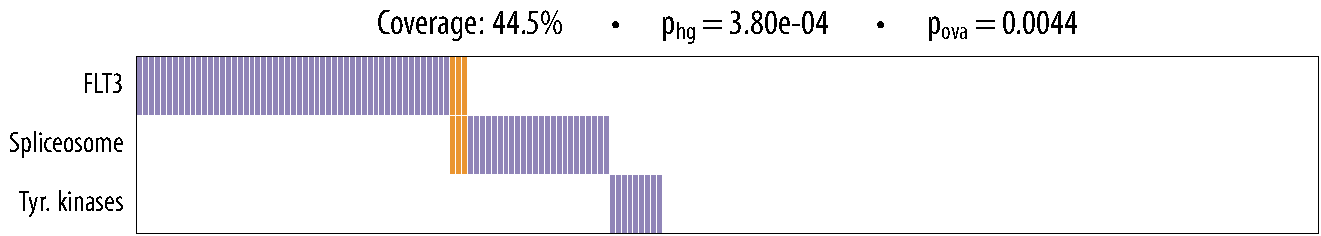
\includegraphics[width=\textwidth]{figures/genes/aml_5.pdf}\\[2em]
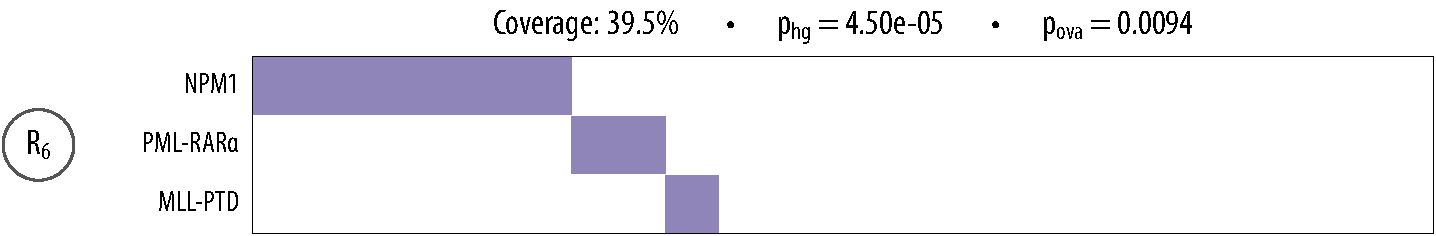
\includegraphics[width=\textwidth]{figures/genes/aml_6.pdf}\\[2em]
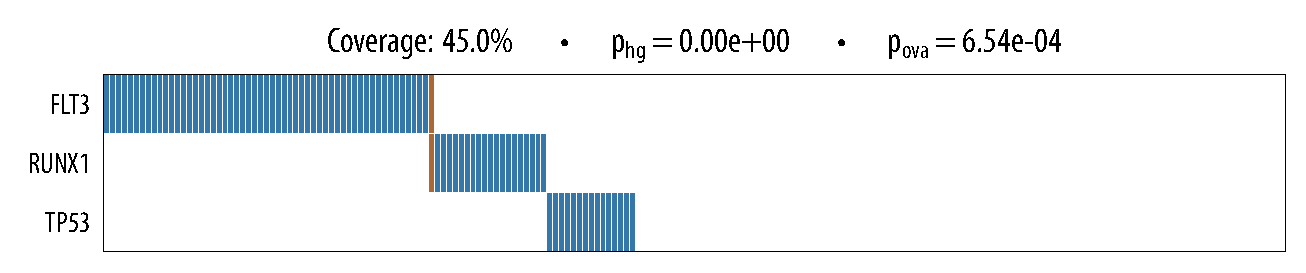
\includegraphics[width=\textwidth]{figures/genes/aml_7.pdf}\\[2em]
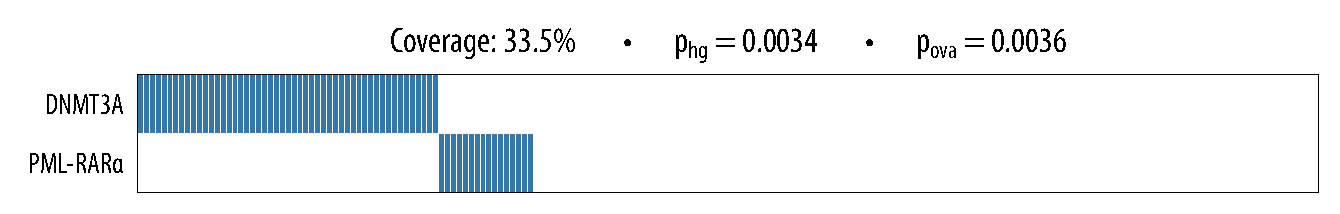
\includegraphics[width=\textwidth]{figures/genes/aml_8.pdf}\\[2em]
\caption{Test}
\end{figure}

\begin{figure}[htb]
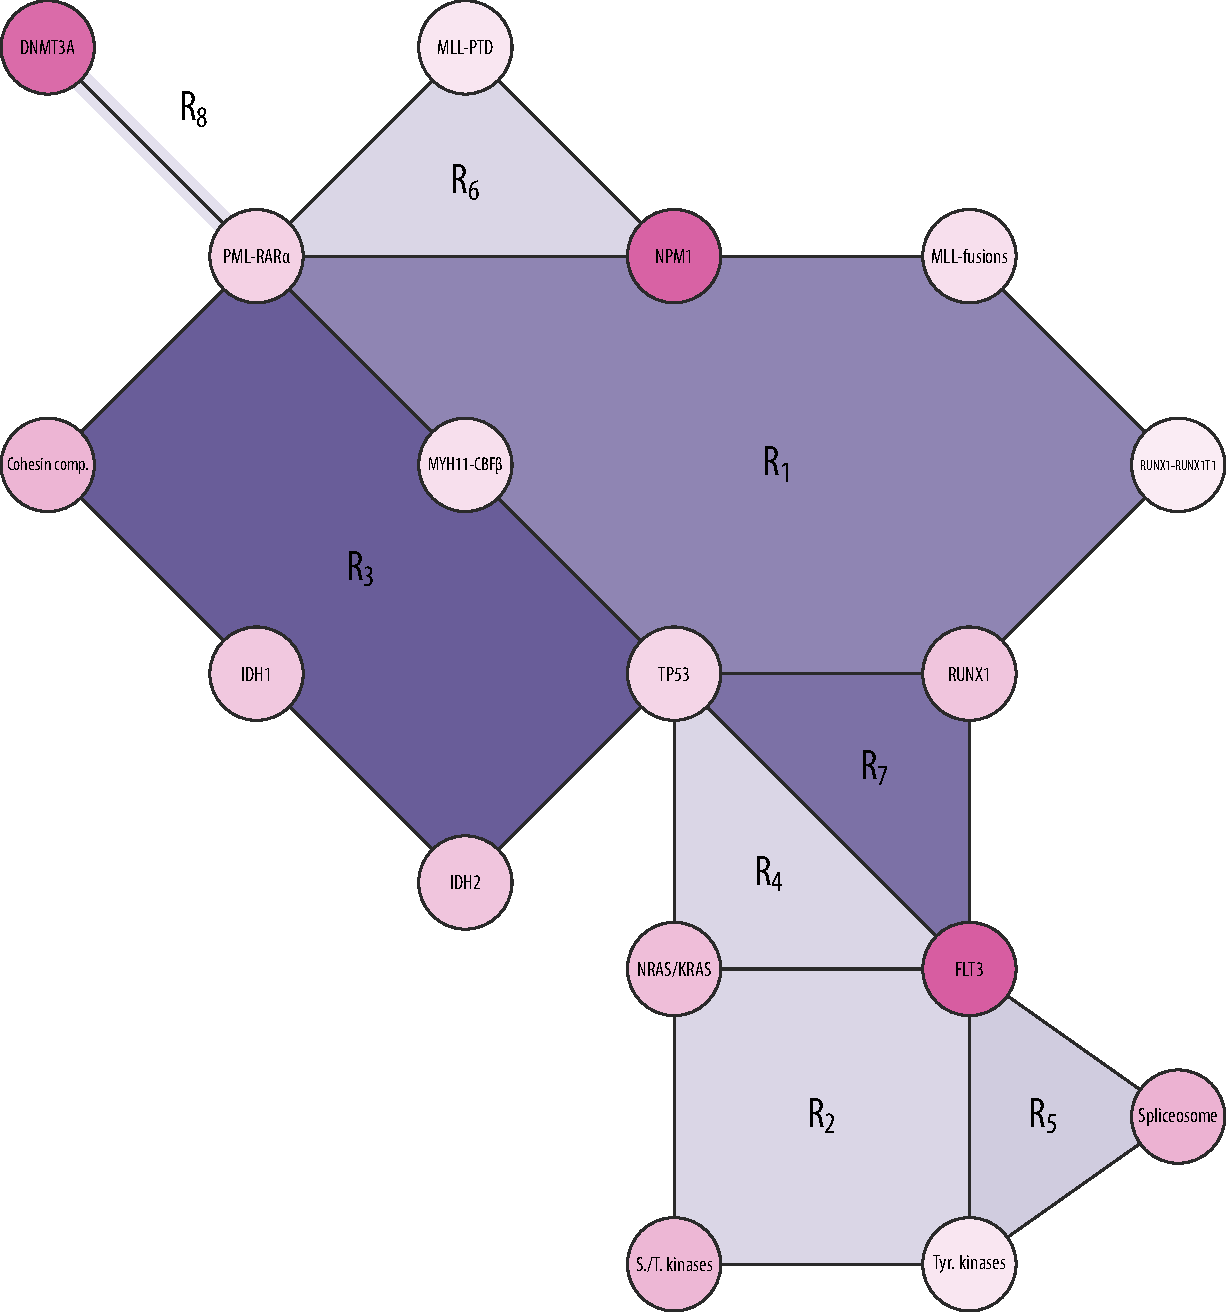
\includegraphics[width=\textwidth]{figures/genes/graph_aml.pdf}\\[2em]
\caption{AML repulsive graph}
\end{figure}

\begin{figure}[htb]
\centering
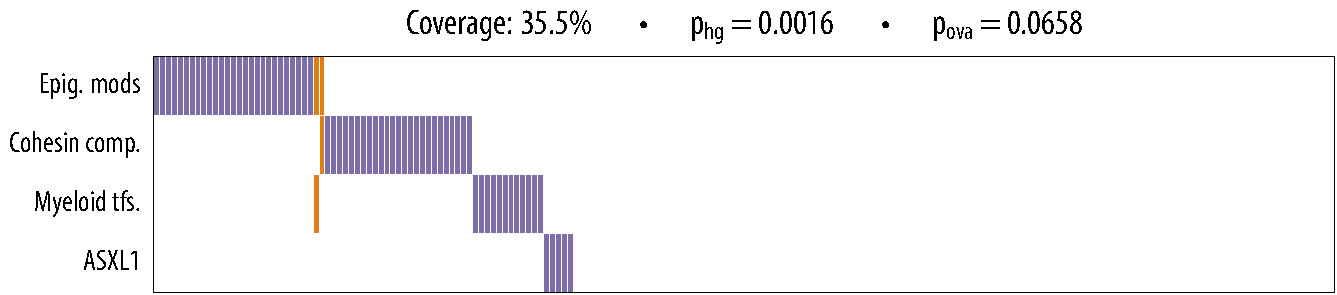
\includegraphics[width=\textwidth]{figures/genes/aml_comet1.pdf}\\[2em]
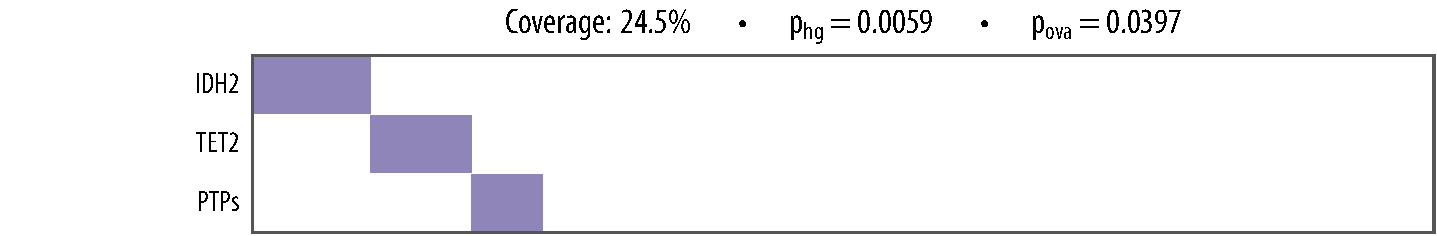
\includegraphics[width=\textwidth]{figures/genes/aml_comet2.pdf}\\[2em]
\caption{CoMEt extra groups (probably appendix)}
\end{figure}

\begin{figure}[htb]
\centering
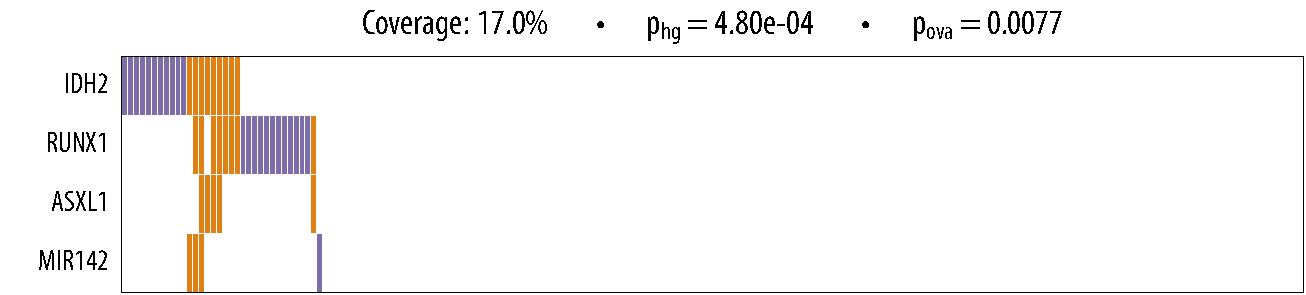
\includegraphics[width=\textwidth]{figures/genes/aml_2_a.pdf}\\[2em]
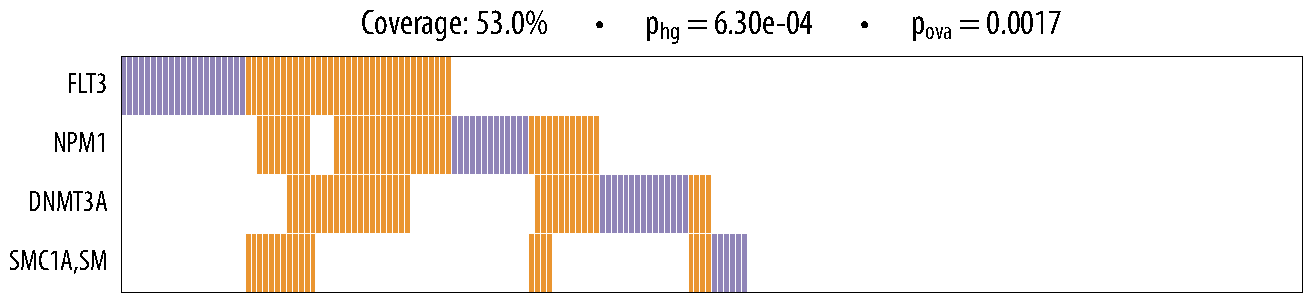
\includegraphics[width=\textwidth]{figures/genes/aml_1_a.pdf}\\[2em]
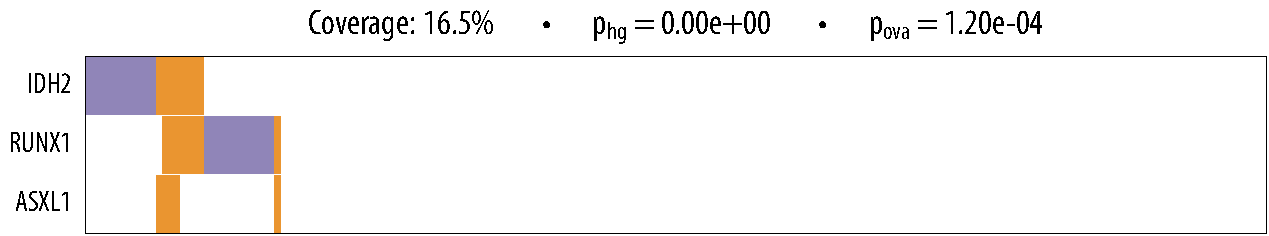
\includegraphics[width=\textwidth]{figures/genes/aml_3_a.pdf}\\[2em]
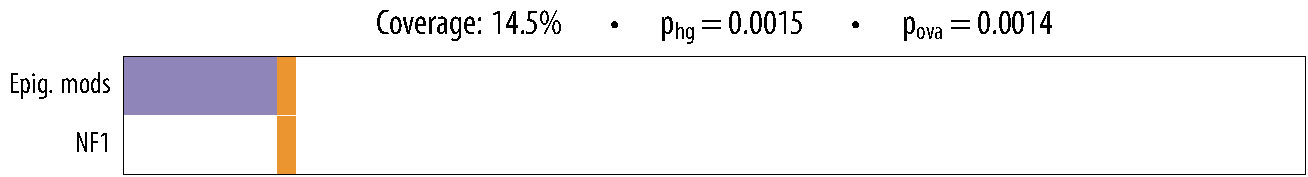
\includegraphics[width=\textwidth]{figures/genes/aml_5_a.pdf}\\[2em]
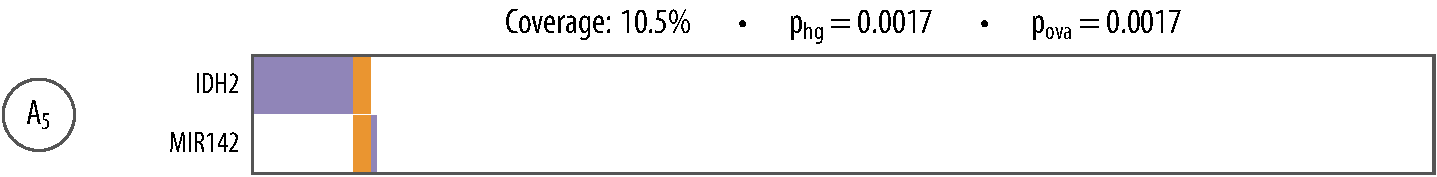
\includegraphics[width=\textwidth]{figures/genes/aml_4_a.pdf}\\[2em]
\caption{Test}
\end{figure}

\subsection{Breast cancer (BRCA)}
\begin{figure}[htb]
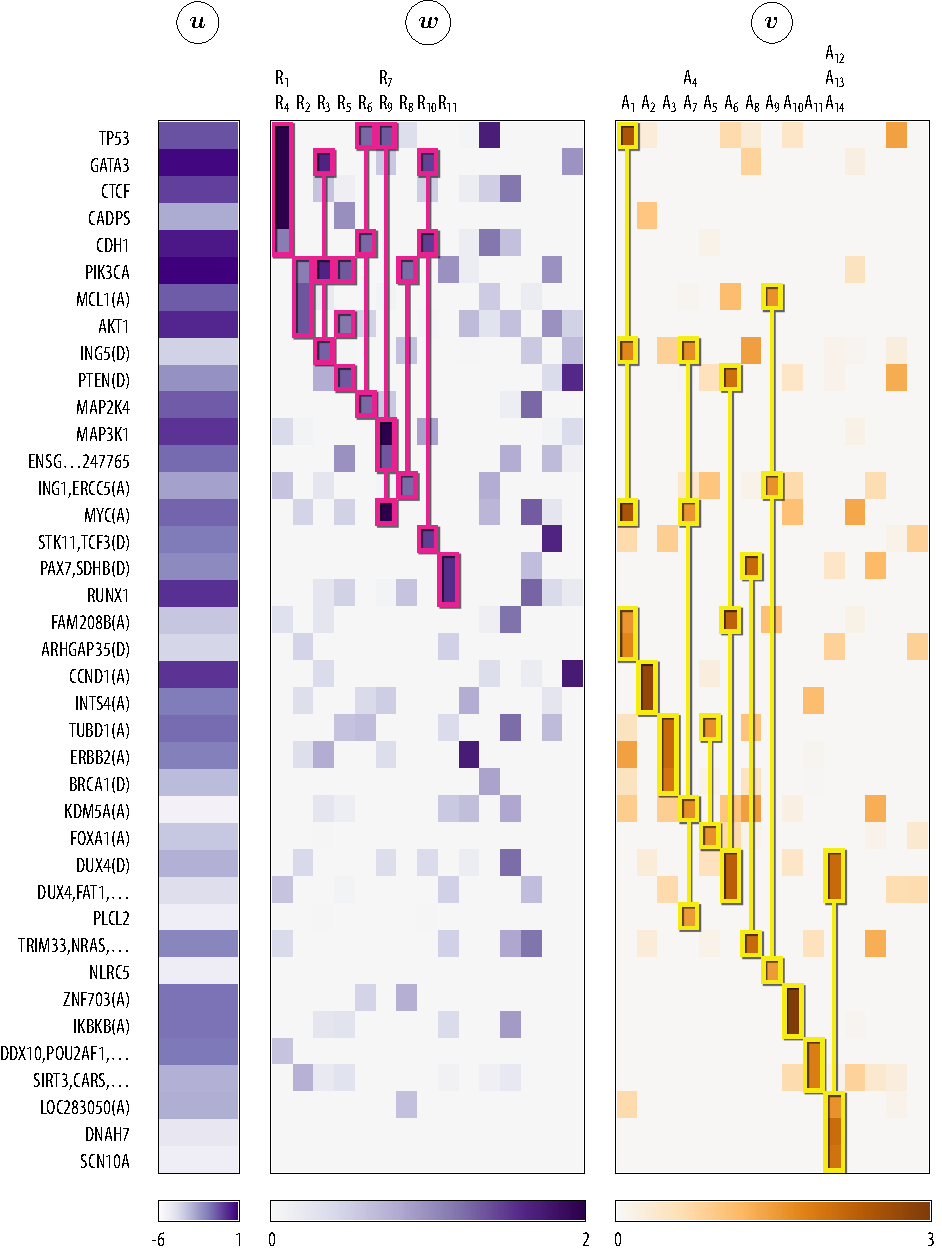
\includegraphics[width=\textwidth]{figures/genes/mat_brca.pdf}\\[2em]
\caption{Test}
\end{figure}

\begin{figure}[htb]
\centering
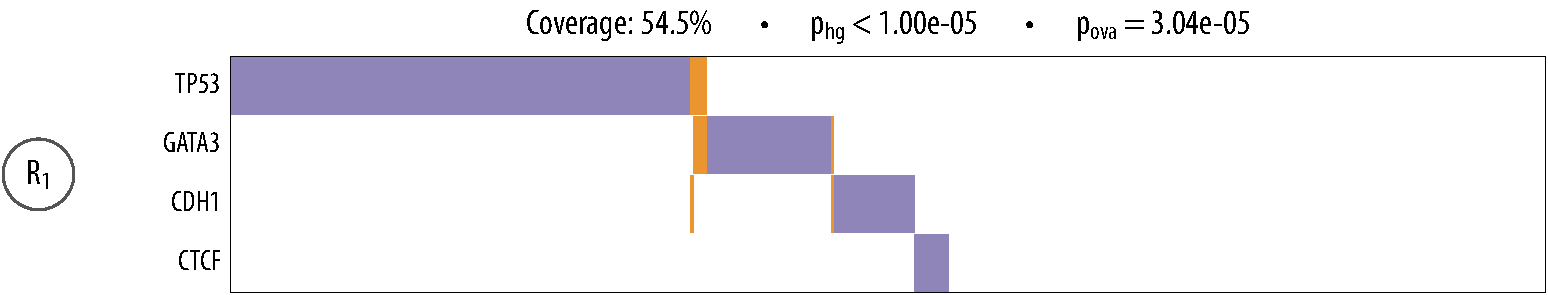
\includegraphics[width=\textwidth]{figures/genes/brca_1.pdf}\\[2em]
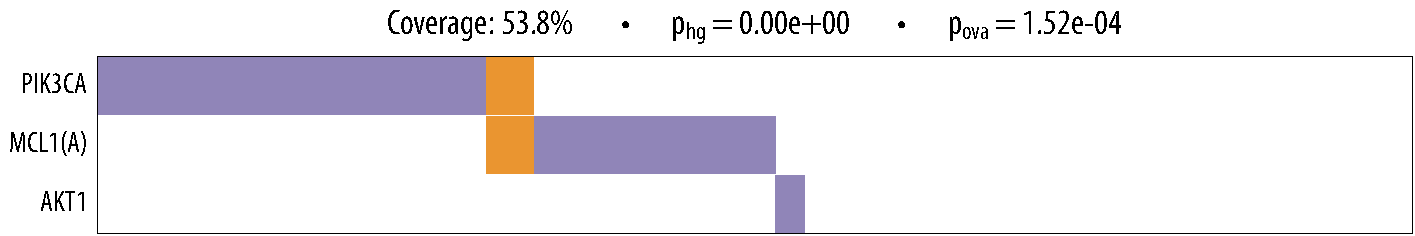
\includegraphics[width=\textwidth]{figures/genes/brca_6.pdf}\\[2em]
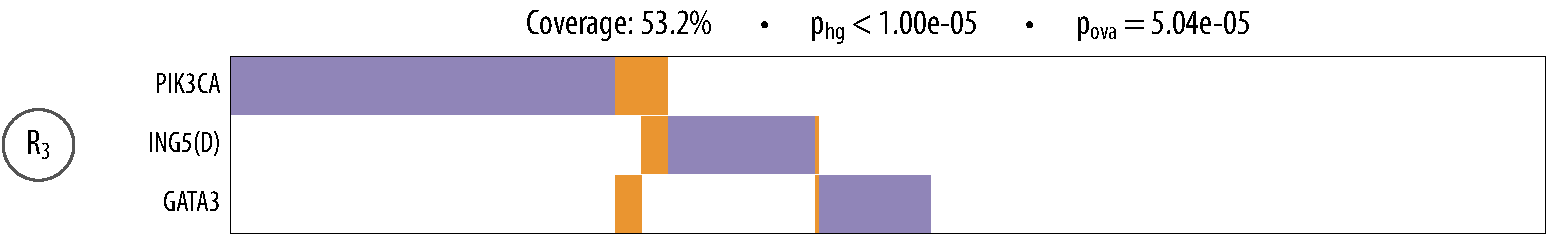
\includegraphics[width=\textwidth]{figures/genes/brca_8.pdf}\\[2em]
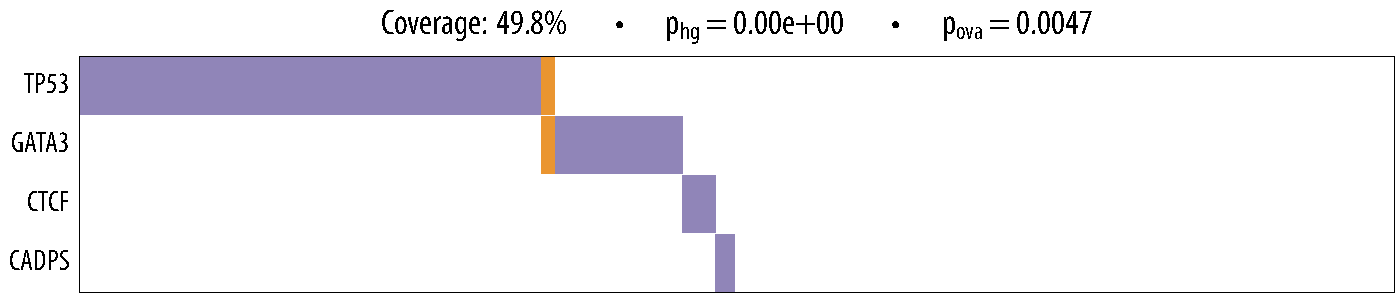
\includegraphics[width=\textwidth]{figures/genes/brca_2.pdf}\\[2em]
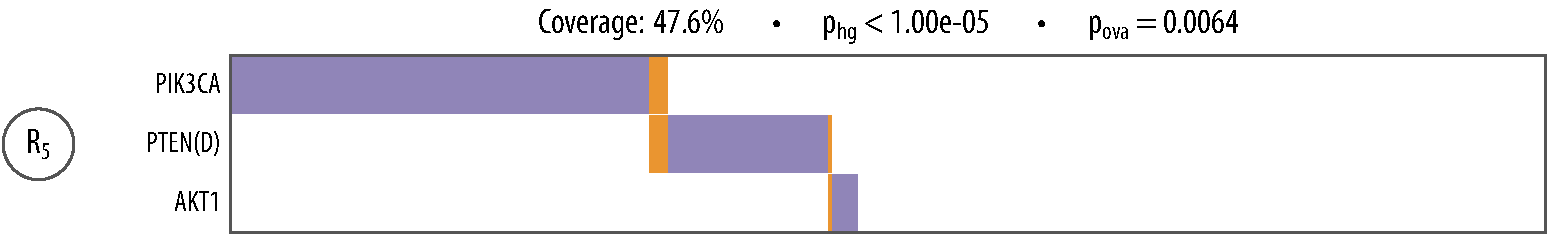
\includegraphics[width=\textwidth]{figures/genes/brca_5.pdf}\\[2em]
\caption{BRCA repulsive (I)}
\end{figure}

\begin{figure}[htb]
\centering
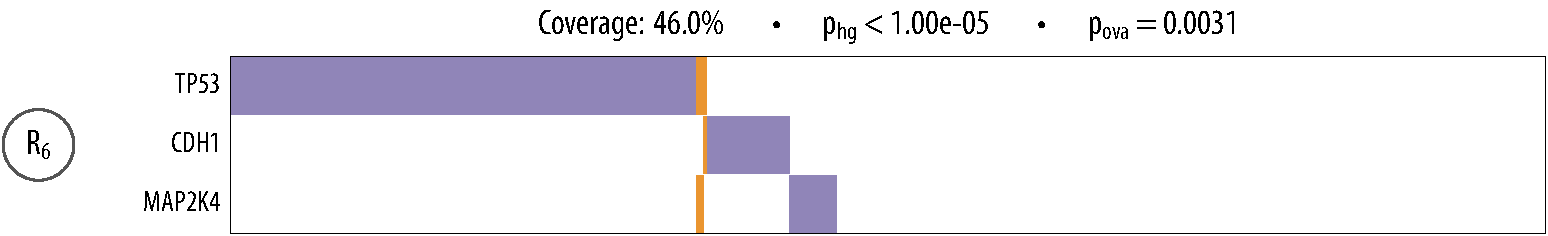
\includegraphics[width=\textwidth]{figures/genes/brca_4.pdf}\\[2em]
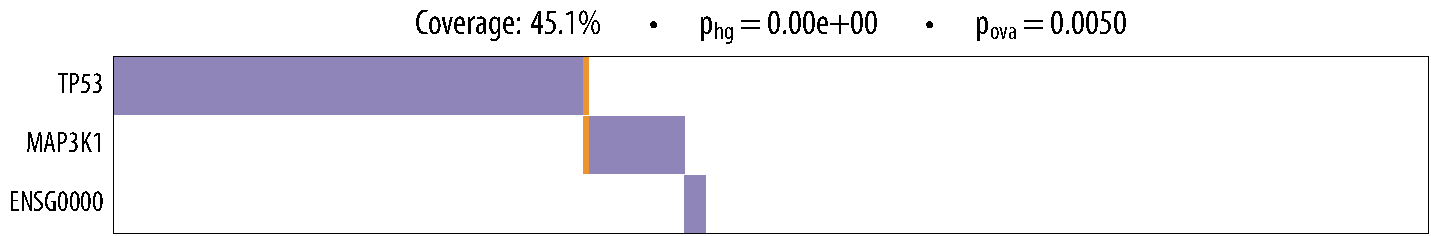
\includegraphics[width=\textwidth]{figures/genes/brca_3.pdf}\\[2em]
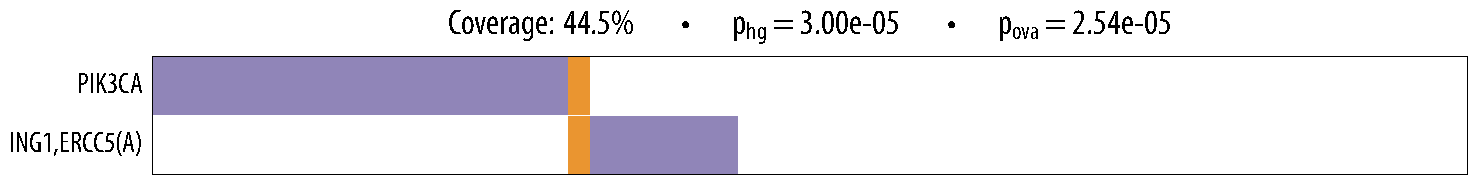
\includegraphics[width=\textwidth]{figures/genes/brca_11.pdf}\\[2em]
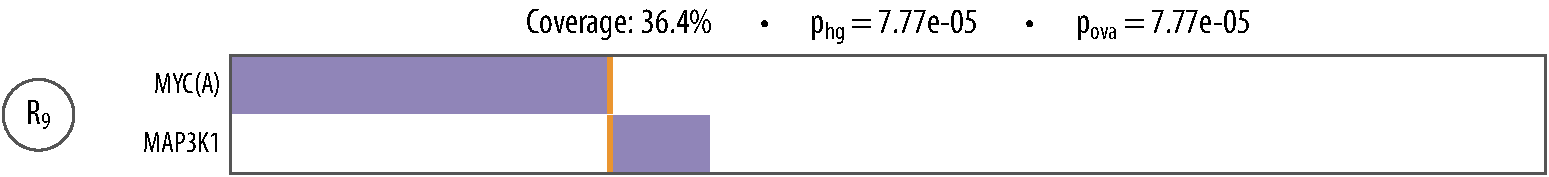
\includegraphics[width=\textwidth]{figures/genes/brca_10.pdf}\\[2em]
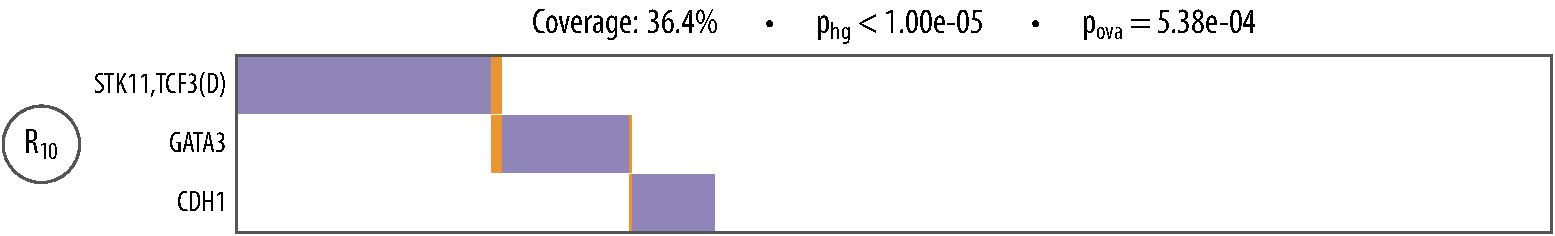
\includegraphics[width=\textwidth]{figures/genes/brca_7.pdf}\\[2em]
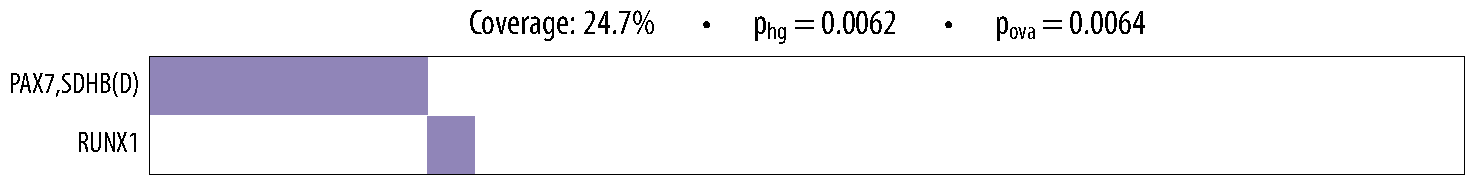
\includegraphics[width=\textwidth]{figures/genes/brca_9.pdf}\\[2em]
\caption{BRCA repulsive (II)}
\end{figure}

\begin{figure}[htb]
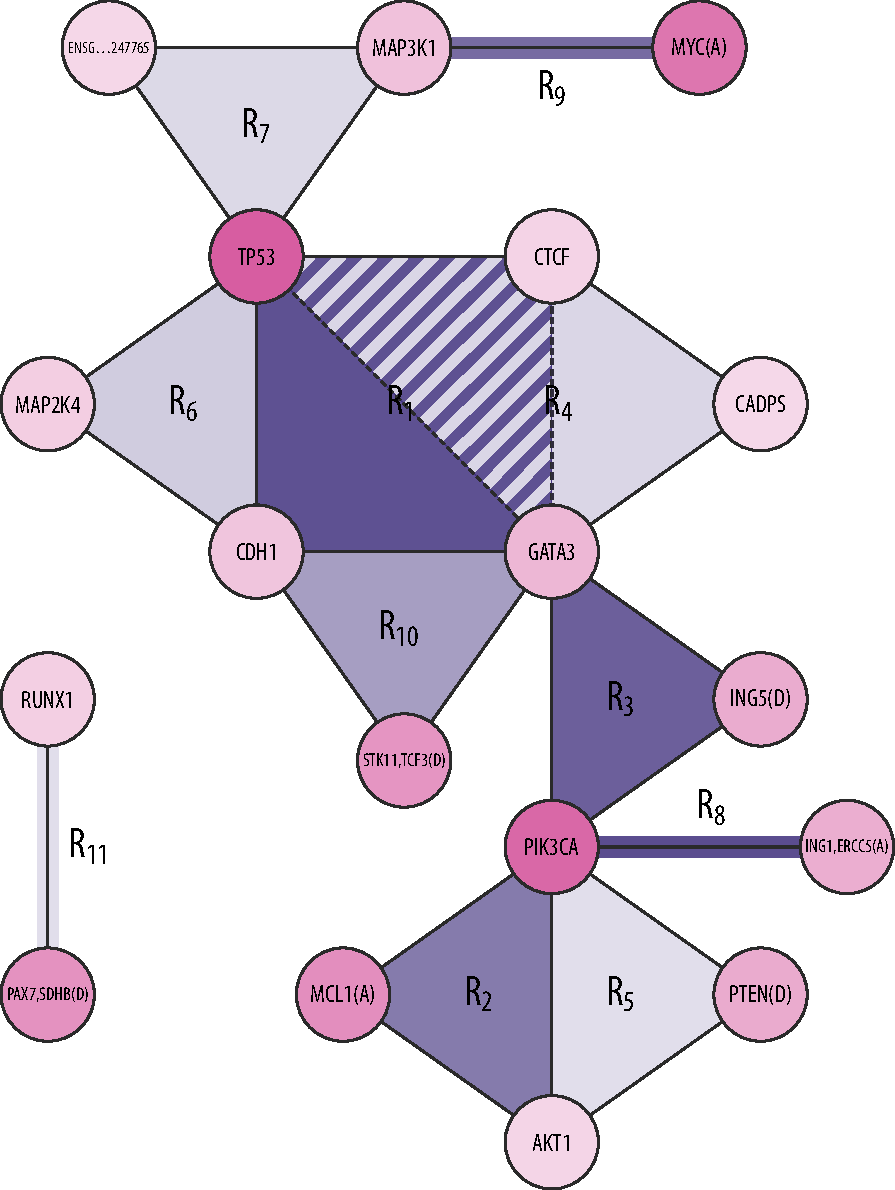
\includegraphics[width=\textwidth]{figures/genes/graph_brca.pdf}\\[2em]
\caption{BRCA repulsive graph}
\end{figure}

\begin{figure}[htb]
\centering
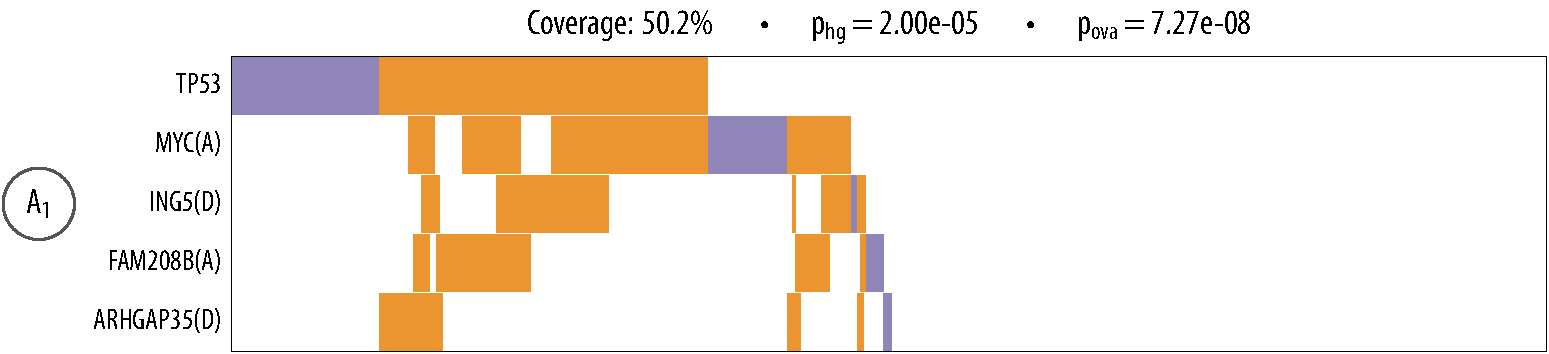
\includegraphics[width=\textwidth]{figures/genes/brca_1_a.pdf}\\[2em]
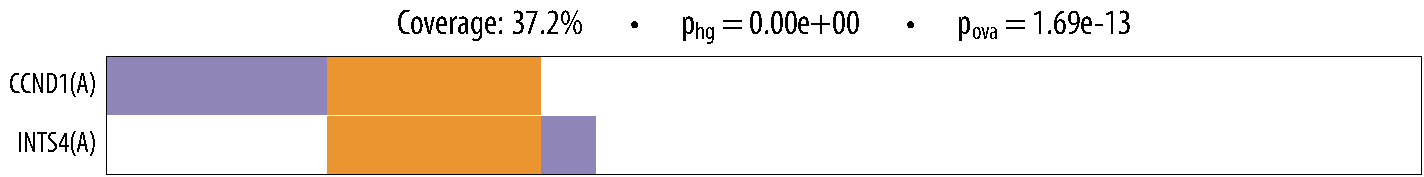
\includegraphics[width=\textwidth]{figures/genes/brca_11_a.pdf}\\[2em]
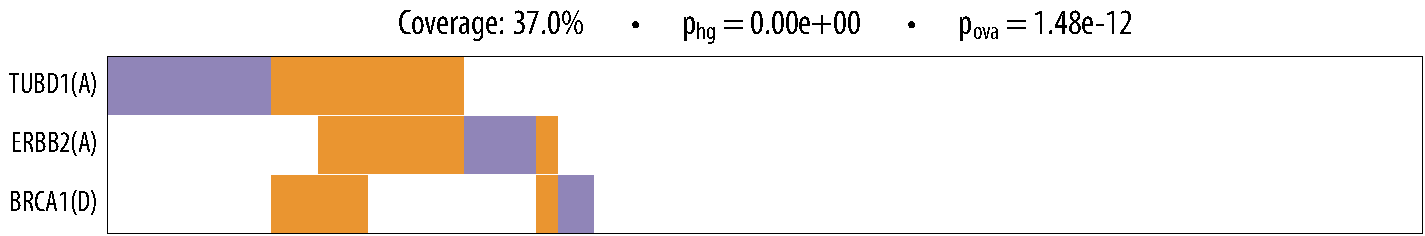
\includegraphics[width=\textwidth]{figures/genes/brca_7_a.pdf}\\[2em]
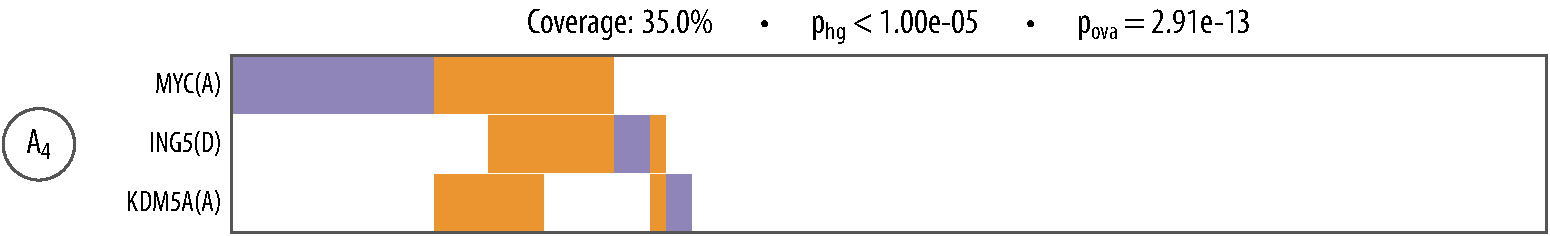
\includegraphics[width=\textwidth]{figures/genes/brca_8_a.pdf}\\[2em]
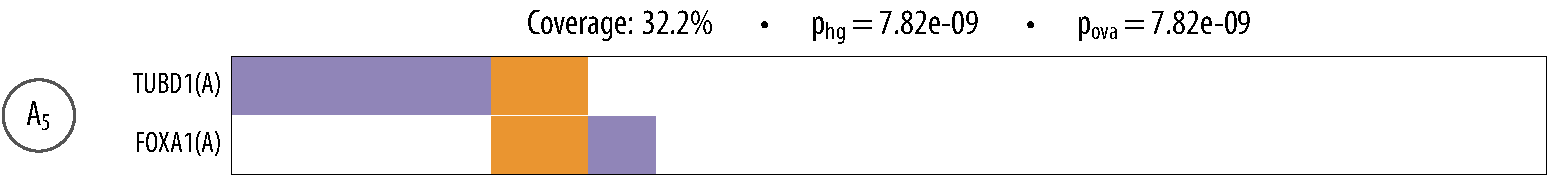
\includegraphics[width=\textwidth]{figures/genes/brca_14_a.pdf}\\[2em]
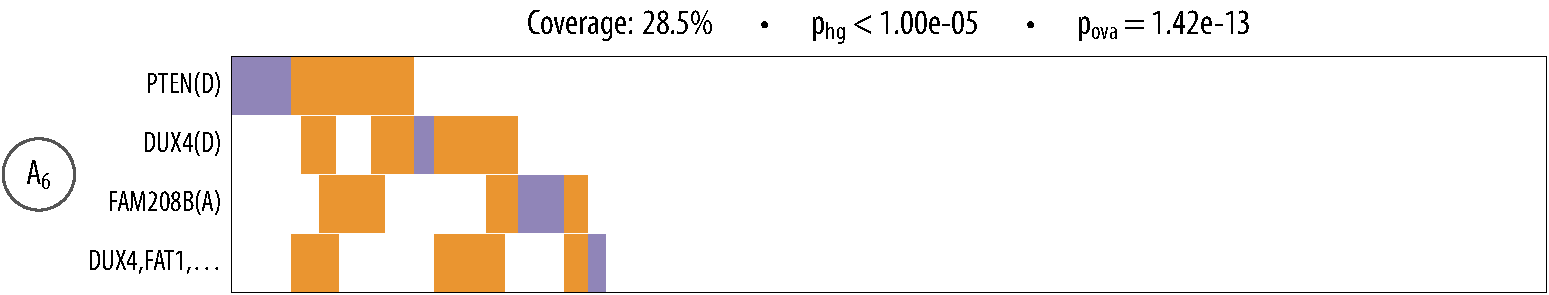
\includegraphics[width=\textwidth]{figures/genes/brca_4_a.pdf}\\[2em]
\caption{BRCA attractive}
\end{figure}

\begin{figure}[htb]
\centering
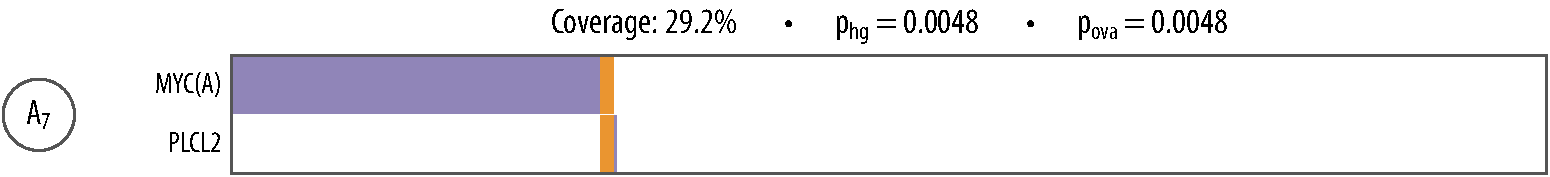
\includegraphics[width=\textwidth]{figures/genes/brca_9_a.pdf}\\[2em]
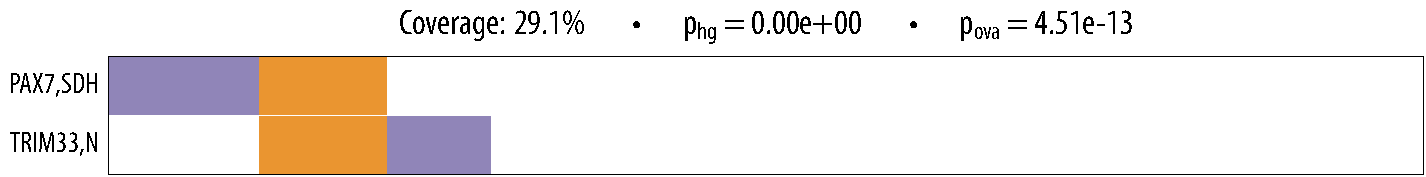
\includegraphics[width=\textwidth]{figures/genes/brca_13_a.pdf}\\[2em]
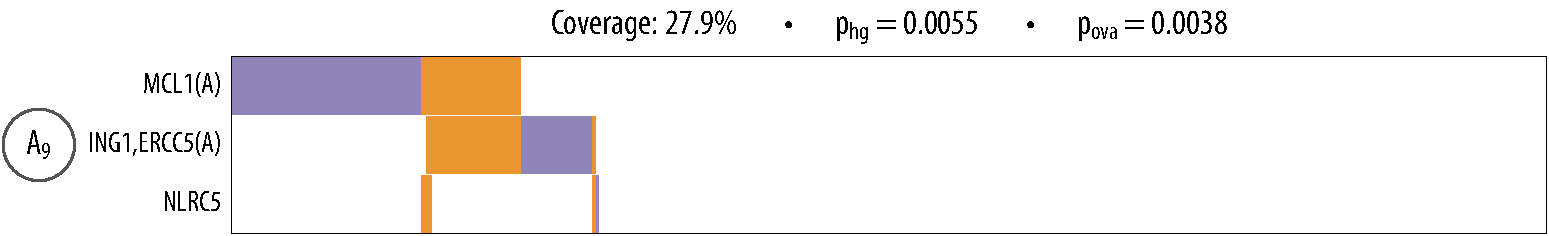
\includegraphics[width=\textwidth]{figures/genes/brca_5_a.pdf}\\[2em]
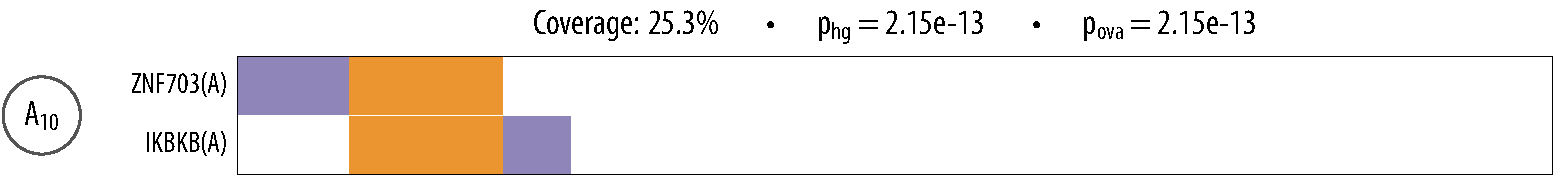
\includegraphics[width=\textwidth]{figures/genes/brca_10_a.pdf}\\[2em]
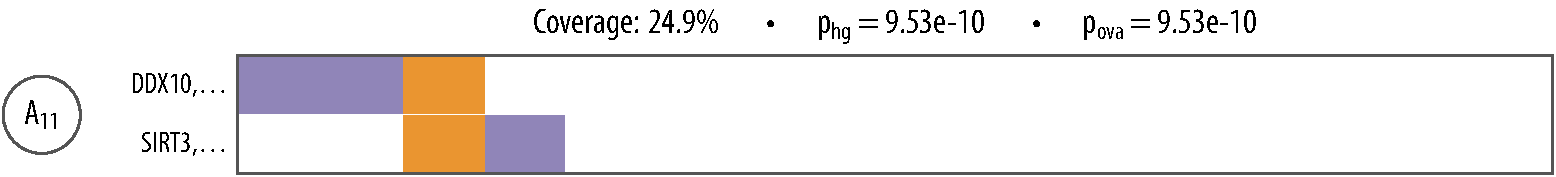
\includegraphics[width=\textwidth]{figures/genes/brca_12_a.pdf}\\[2em]
\caption{BRCA attractive (appendix I)}
\end{figure}

\begin{figure}[htb]
\centering
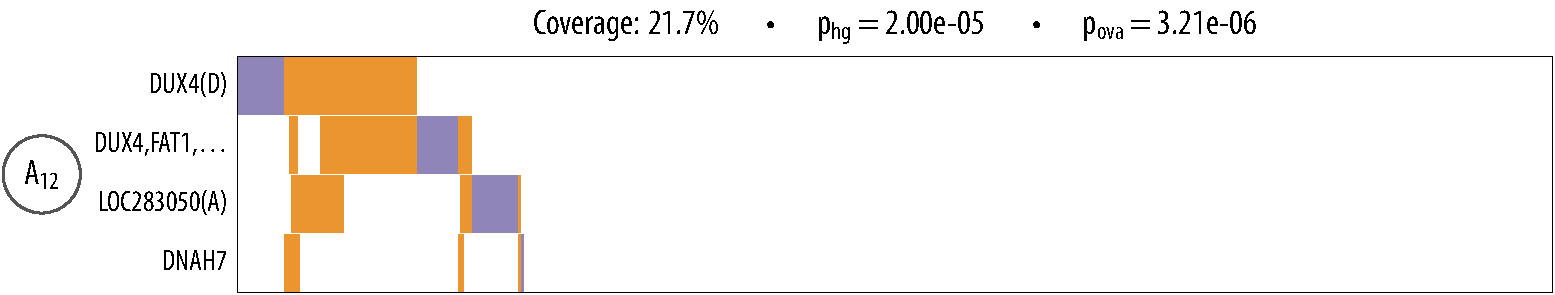
\includegraphics[width=\textwidth]{figures/genes/brca_3_a.pdf}\\[2em]
%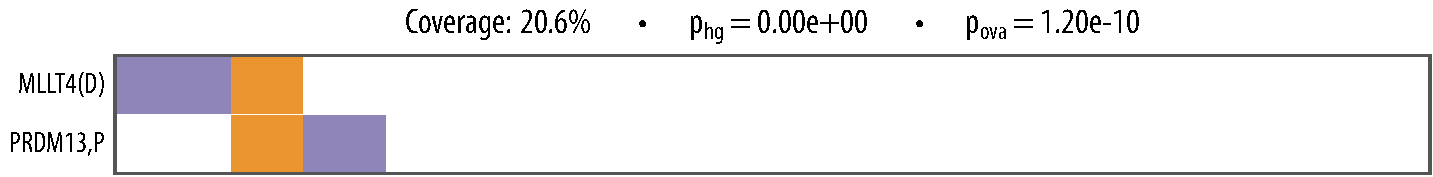
\includegraphics[width=\textwidth]{figures/genes/brca_15_a.pdf}\\[2em]
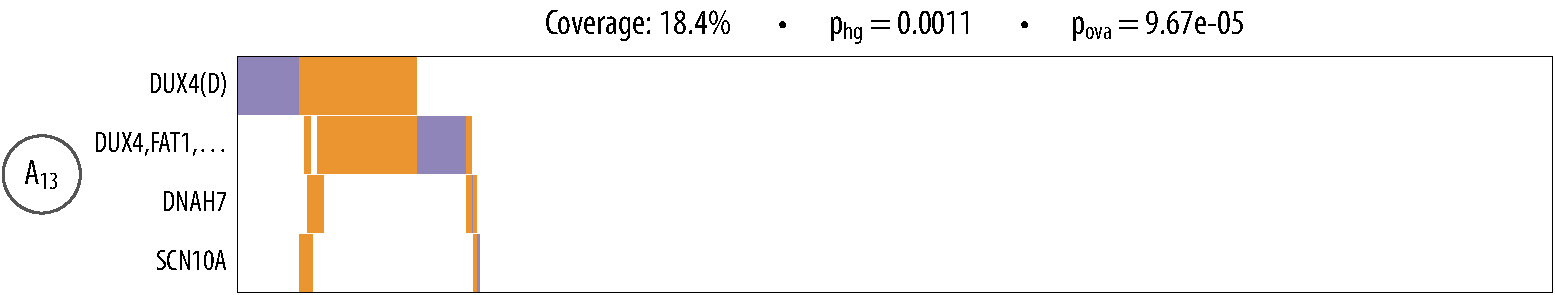
\includegraphics[width=\textwidth]{figures/genes/brca_2_a.pdf}\\[2em]
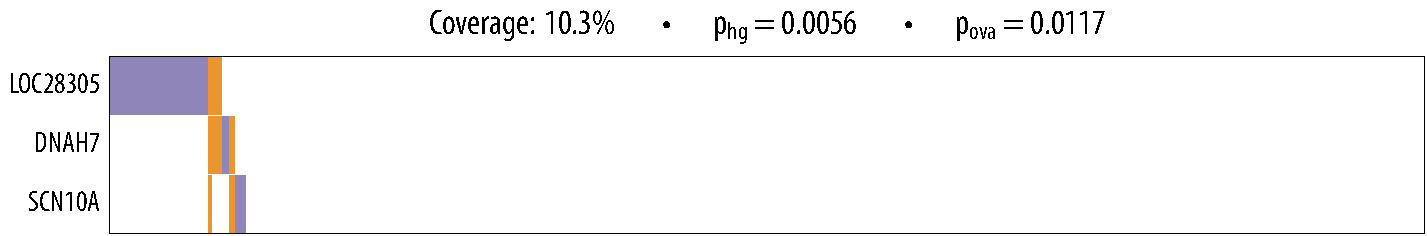
\includegraphics[width=\textwidth]{figures/genes/brca_6_a.pdf}\\[2em]
\caption{BRCA attractive (appendix II)}
\end{figure}

\section{Conclusion}